\achapter{7}{Matrix Transformations} \label{sec:matrix_transformations}

\vspace*{-17 pt}
\framebox{
\parbox{\dimexpr\linewidth-3\fboxsep-3\fboxrule}
{\begin{fqs}
\item What is a matrix transformation? 
\item What properties do matrix transformations have? (In particular, what properties make matrix transformations \emph{linear}?)
\item What is the domain of a matrix transformation defined by an $m \times n$ matrix? Why? 
\item What are the range and codomain of a matrix transformation defined by an $m \times n$ matrix? Why? 
\item What does it mean for a matrix transformation to be one-to-one? If $T$ is a matrix transformation represented as $T(\vx) = A \vx$, what are the conditions on $A$ that make $T$ a one-to-one transformation? 
\item What does it mean for a matrix transformation to be onto? If $T$ is a matrix transformation represented as $T(\vx) = A \vx$, what are the conditions on $A$ that make $T$ an onto transformation?
\end{fqs}}}% \hspace*{3 pt}}

\vspace*{13 pt}

\csection{Application: Computer Graphics}

As we will discuss, left multiplication by an $m \times n$ matrix defines a function from $\R^n$ to $\R^m$. Such a function defined by matrix multiplication is called a matrix transformation. In this section we study some of the properties of matrix transformations and understand how, using the pivots of the matrix, to determine when the output of a matrix transformation covers the whole space $R^m$ or when a transformation maps distinct vectors to distinct outputs. 

Matrix transformations are used extensively in computer graphics to produce animations as seen in video games and movies. For example, consider the dancing figure at left in Figure \ref{F:Rotate_dance}. We can identify certain control points (e.g., the point at the neck, where the arms join the torso, etc.) to mark the locations of important points. Using just the control points we can reconstruct the figure. Each control point can be represented as a vector, and so we can manipulate the figure by manipulating the control points with matrix transformations. We will explore this idea in more detail later in this section. 

\begin{figure}[ht]
\begin{center}
\resizebox{!}{1.5in}{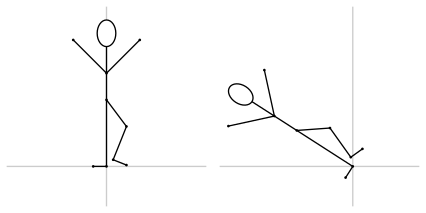
\includegraphics{1_g_dancer_rotate}} 
%\resizebox{!}{1.5in}{\includegraphics{Dancing_man_original}} \hspace{0.5in}  \resizebox{!}{1.5in}{\includegraphics{Dancing_man_rotate}}
\caption{A dancing figure and a rotated dancing figure.}
\label{F:Rotate_dance}
\end{center}
\end{figure}

\csection{Introduction}

In this section we will consider special functions which take vectors as inputs and produce vectors as outputs. We will use matrix multiplication to produce the output vectors.

If $A$ is an $m \times n$ matrix and $\vx$ is a vector in $\R^n$, then the matrix-vector product $A \vx$ is a vector in $\R^m$. (Pick some specific $n, m$ values to understand this statement better.) Therefore, left multiplication by the matrix $A$ takes an input vector $\vx$ in $\R^n$ and produces an output vector $A\vx$ in $\R^m$, which we will refer to as the \emph{image} of $\vx$ under the transformation. This defines a function $T$ from $\R^n$ to $\R^m$ where
\[ T(\vx) = A \vx \, .\]
These functions are the matrix transformations. 

\begin{definition} A \textbf{matrix transformation}\index{matrix transformation}\index{transformation!matrix} is a function $T: \R^n \to \R^m$ defined by 
\[T(\vx) = A\vx\]
for some $m \times n$ matrix $A$. 
\end{definition}

Many of the transformations we consider in this section are from $\R^2$ to $\R^2$ so that we can visualize the transformations.  As an example, let us consider the transformation $T$ defined by 
\[T\left(\left[ \begin{array}{c} x_1 \\ x_2 \end{array} \right] \right) = \left[ \begin{array}{cr} 1&0 \\ 0&-1 \end{array} \right]\left[ \begin{array}{c} x_1 \\ x_2 \end{array} \right]. \]

If we plot the input vectors $\vu_1 = \left[ \begin{array}{c}  1 \\ 0 \end{array} \right]$, $\vu_2 = \left[ \begin{array}{c}  0\\1 \end{array} \right]$, $\vu_3 = \left[ \begin{array}{c} 1  \\ 2 \end{array} \right]$, and  $\vu_4 = \left[ \begin{array}{r} -1  \\ 1 \end{array} \right]$ (as (blue) circles) and their images $T(\vu_1) = \left[ \begin{array}{cr} 1&0 \\ 0&-1 \end{array} \right]\left[ \begin{array}{c} 1 \\ 0 \end{array} \right] = \left[ \begin{array}{c} 1 \\ 0 \end{array} \right]$, $T(\vu_2) = \left[ \begin{array}{r} 0 \\ -1 \end{array} \right]$, $T(\vu_3) = \left[ \begin{array}{r} 1 \\ -2 \end{array} \right]$, and $T(\vu_4) = \left[ \begin{array}{r} -1 \\ -1 \end{array} \right]$ (as (red) $\times$'s) on the same set of axes as shown in Figure \ref{F:PA_1g_1}, we see that this transformation reflects the input vectors across the $x$-axis. We can also see this algebraically since the reflection of the point $(x_1,x_2)$ around the $x$-axis is the point $(x_1,-x_2)$, and 
\[T\left( \left[ \begin{array}{c} x_1 \\ x_2 \end{array} \right] \right) = \left[ \begin{array}{r} x_1 \\ -x_2 \end{array} \right].\]

\begin{figure}[ht]
\begin{center}
\resizebox{!}{3.0in}{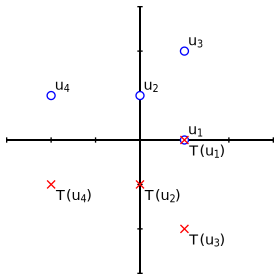
\includegraphics{1g_pa1_b}}
\caption{Inputs and outputs of the transformation $T$.}
\label{F:PA_1g_1}
\end{center}
\end{figure}	

\begin{pa} \label{pa:1_g} We now consider other transformations from $\R^2$ to $\R^2$. 

\be	
\item Suppose a transformation $T$ is defined by 
\[T\left( \left[ \begin{array}{c}  x_1\\x_2 \end{array} \right] \right) = \left[ \begin{array}{cc} 2&0 \\ 0&2 \end{array} \right] \left[ \begin{array}{c}  x_1 \\ x_2 \end{array} \right].\]
	\ba
	\item Find $T(\vu_i)$ for each of $\vu_1 = \left[ \begin{array}{c}  1 \\ 0 \end{array} \right]$, $\vu_2 = \left[ \begin{array}{c}  0\\1 \end{array} \right]$, $\vu_3 = \left[ \begin{array}{c} 1  \\ 2 \end{array} \right]$, and  $\vu_4 = \left[ \begin{array}{r} -1  \\ 1 \end{array} \right]$. (In other words, substitute $\vu_1, \vu_2, \vu_3, \vu_4$ into the formula above to see what output is obtained.)

	\item Plot all input vectors and their images on the same axes in $\R^2$. Clearly identify which image corresponds to which input vector. Then give a geometric description of what this transformation does. 


	\ea
	
\item The transformation in the introduction performs a reflection across the $x$-axis. Find a matrix transformation that performs a reflection across the $y$-axis.

	
\item Suppose a transformation $T$ is defined by 
\[T(\vx) = A\vx,\]
where 
\[A = \left[ \begin{array}{cc} 1&0 \\ 0&0 \end{array} \right].\]
	\ba
	\item Find $T(\vu_i)$ for each of $\vu_1 = \left[ \begin{array}{c}  1 \\ 0 \end{array} \right]$, $\vu_2 = \left[ \begin{array}{c}  0\\1 \end{array} \right]$, $\vu_3 = \left[ \begin{array}{c} 1  \\ 2 \end{array} \right]$, and  $\vu_4 = \left[ \begin{array}{r} -1  \\ 1 \end{array} \right]$. 


	\item Plot all input vectors and their images on the same axes in $\R^2$. Give a geometric description of this transformation.

	\item Is there an input vector which produces $\vb = \left[ \begin{array}{c}  1 \\ 1 \end{array} \right]$ as an output vector?


	\item Find all input vectors that produce the output vector $\vb = \left[ \begin{array}{c}  1 \\ 0 \end{array} \right]$. Is there a unique input vector, or multiple input vectors? 

	\ea
	

\ee
\end{pa}


\csection{Properties of Matrix Transformations}

A matrix transformation is a function. When dealing with functions in previous mathematics courses we have used the terms domain and range with our functions. Recall that the domain of a function is the set of all allowable inputs into the function and the range of a function is the set of all outputs of the function. We do the same with transformations. If $T$ is the matrix transformation $T(\vx) = A \vx$ for some $m \times n$ matrix $A$, then $T$ maps vectors from $\R^n$ into $\R^m$. So $\R^n$ is the \emph{domain}\index{domain of a matrix transformation} of $T$ -- the set of all input vectors. However, the set $\R^m$ is only the target set for $T$ and not necessarily the range of $T$.  We call $\R^m$ the \emph{codomain}\index{codomain of a matrix transformation}  of $T$, while the \emph{range}\index{range of a matrix transformation} of $T$ is the set of all output vectors. The range of a transformation will come up later, so we make a formal definition.

\begin{definition} The \textbf{range}\index{range of a matrix transformation} of a matrix transformation $T$ from $\R^n$ to $\R^m$ is the set 
\[\Range{T} = \{T(\vx) : \vx \in \R^n\}.\]
\end{definition}

The range is always a subset of the codomain, but the two sets do not have to be equal. In addition, if a vector $\vb$ in $\R^m$ satisfies $\vb = T(\vx)$ for some $\vx$ in $\R^n$, then we say that $\vb$ is the \emph{image}\index{image of an element under a transformation} of $\vx$ under the transformation $T$. For this reason we also use the term \emph{image}\index{image of a matrix transformation} to also mean the range of a transformation, with the corresponding notation $\Image(T)$. 



Because of the properties of the matrix-vector product, if the matrix transformation $T$ is defined by $T(\vx) = A\vx$ for some $m \times n$ matrix $A$, then 
\[T(\vu + \vv) =  A(\vu + \vv) = A\vu + A\vv\]
and 
\[T(c\vu) = A(c\vu) = cA\vu = cT(\vu)\]
for any vectors $\vu$ and $\vv$ in $\R^n$ and any scalar $c$. So every matrix transformation $T$ satisfies the following two important properties:
\begin{enumerate}
\item $T(\vu + \vv) =  T(\vu) + T(\vv)$ and
\item $T(c\vu) = c T(\vv)$.
\end{enumerate}
The first property says that a matrix transformation $T$ preserves sums of vectors and the second that $T$ preserves scalar multiples of vectors. 


\begin{activity} \label{act:1_g_2} Let $T$ be a matrix transformation, and let $\vu$ and $\vv$ be vectors in the domain of $T$ so that $T(\vu) = \left[ \begin{array}{c} 1 \\ 2 \\  0 \end{array} \right]$ and $T(\vv) = \left[ \begin{array}{r} -3 \\ 1 \\  4 \end{array} \right]$. 
\ba
\item Exactly which vector is $T(2\vu - 3\vv)$? Explain.

\item If $a$ and $b$ are any scalars, what is the vector $T(a\vu + b\vv)$? Why? 

\ea

\end{activity}


As we saw in Activity \ref{act:1_g_2}, we can combine the two properties of a matrix transformation $T$ into one: for any scalars $a$ and $b$ and any vectors $\vu$ and $\vv$ in the domain of $T$ we have  
\begin{equation} \label{eq:1_g_1}
T(a\vu+b\vv) = aT(\vu) + bT(\vv).
\end{equation}
 We can then extend equation (\ref{eq:1_g_1}) (by mathematical induction) to any finite linear combination of vectors. That is, if $\vv_1$, $\vv_2$, $\ldots$, $\vv_k$ are any vectors in the domain of a matrix transformation $T$ and if $x_1$, $x_2$, $\ldots$, $x_k$ are any scalars, then
\begin{equation} \label{eq:1_g_2}
T(x_1 \vv_1 + x_2 \vv_2 + \cdots + x_k \vv_k) = x_1 T(\vv_1) + x_2 T(\vv_2) + \cdots + x_k T(\vv_k).
\end{equation}
In other words, a matrix transformation preserves linear combinations. For this reason matrix transformations are examples of a larger set of transformation that are called \emph{linear} transformations. We will discuss general linear transformations in a later section.
 

There is one other important property of a matrix transformation for us to consider. The functions we encountered in earlier mathematics courses, e.g., $f(x) = 2x+1$, could send the input 0 to any output. However, as a consequence of the definition, any matrix transformation $T$ maps the zero vector to the zero vector because
\[ T(\vzero) = A\vzero = \vzero \,.\]

Note that the two vectors $\vzero$ in the last equation may not be the same vector -- if $T : \R^n \to \R^m$, then the first $\vzero$ is in $\R^n$ and the second in $\R^m$. It should be clear from the context which vector $\vzero$ is meant. 


\csection{Onto and One-to-One Transformations}

The problems we have been asking about solutions to systems of linear equations can be rephrased in terms of matrix transformations. The question about whether a system $A \vx = \vb$ is consistent for any vector $\vb$ is also a question about the existence of a vector $\vx$ so that $T(\vx) = \vb$, where $T$ is the matrix transformation defined by $T(\vx) = A \vx$. 


\begin{activity} \label{act:1_g_4} Let $T$ be the matrix transformation defined by $T(\vx) = A\vx$ where $A$ is 
\[\left[ \begin{array}{rc} 1&0 \\ 0&1 \\ 0&2 \end{array} \right].\] 
\ba
\item Find $T\left(\left[\begin{array}{c} 1\\1\end{array}\right]\right)$ and $T\left(\left[\begin{array}{c} 1\\1\\1\end{array}\right]\right)$. If it is not possible to find one or both of the output vectors, indicate why.


\item What are the domain and codomain of $T$? Why? (Recall that the domain is the space of all input vectors, while the codomain is the space in which the output vectors are contained.)

\item Can you find a vector $\vx$ for which $T(\vx)= \left[\begin{array}{c} 2\\3\\6\end{array}\right]$? Can you find a vector $\vx$ for which $T(\vx)=\left[\begin{array}{c} 2\\3\\1\end{array}\right]$?

\item Which $\vb=\left[\begin{array}{c} a\\b\\c\end{array}\right]$ are the image vectors for this transformation? Is the range of $T$ equal to the codomain of $T$? Explain. 
 
\item The previous question can be rephrased as a matrix equation question.  We are asking whether $A \vx = \vb$ is consistent for every $\vb$. How is the answer to this question related to the pivots of $A$? 

\ea

\end{activity}


If $T$ is a matrix transformation, Activity \ref{act:1_g_4} illustrates that the range of a matrix transformation $T$ may not equal its codomain. In other words, there may be vectors $\vb$ in the codomain of $T$ that are not the image of any vector in the domain of $T$. If it is the case for a matrix transformation $T$ that there is always a vector $\vx$ in the domain of $T$ such that $T(\vx) = \vb$ for any vector $\vb$ in the codomain of $T$, then $T$ is given a special name.

\begin{definition} A matrix transformation $T$ from $\R^n$ to $\R^m$ is \textbf{onto}\index{onto} if each $\vb$ in $\R^m$ is the image of \emph{at least one} $\vx$ in $\R^n$.
\end{definition}   


So the matrix transformation $T$ from $\R^n$ to $\R^m$ defined by $T(\vx) = A\vx$ is onto if the equation $A \vx = \vb$ has a solution for each vector $\vb$ in $\R^m$. Since the vectors $A\vx$ are linear combinations of the columns of $A$, $T$ is onto exactly when the span of the columns of $A$ is all of $\R^m$. Activity \ref{act:1_g_4} shows us that $T$ is onto if every row of $A$ contains a pivot. 

Another question to ask about matrix transformations is how many vectors there can be that map onto a given output vector.


\begin{activity} \label{act:1_g_5} Let $T$ be the matrix transformation defined by $T(\vx) = A \vx$ where $A$ is 	
\[\left[ \begin{array}{ccc} 1 & 3 & 0 \\ 0 & 0 & 1 \end{array} \right].\]
\ba
\item Find $T\left(\left[\begin{array}{c} 1\\1\end{array}\right]\right)$ and $T\left(\left[\begin{array}{c} 1\\1\\1\end{array}\right]\right)$. If it is not possible to find one or both of the output vectors, indicate why.


\item What are the domain and codomain of $T$? Why?


\item Find $T\left(\left[\begin{array}{c} 1\\1\\2\end{array}\right]\right)$. Are there any other $\vx$'s for which $T(\vx)$ is this same output vector? (Hint: Set up an equation to solve for such $\vx$'s.)
  
\item Assume more generally that for some vector $\vb$, there is a vector $\vx$ so that $T(\vx) = \vb$. Write this as a matrix equation to determine how many solutions this equation has. Explain. How is the answer to this question related to the pivots of $A$?

\ea

\end{activity}


The uniqueness of a solution to $A \vx = \vb$ is the same as saying that the matrix transformation $T$ defined by $T(\vx) = A\vx$ maps exactly one vector to $\vb$. A matrix transformation $T$ that has the property that every image vector is an image in exactly one way is also a special type of transformation.


\begin{definition} A matrix transformation $T$ from $\R^n$ to $\R^m$ is \textbf{one-to-one}\index{one-to-one} if each $\vb$ in $\R^m$ is the image of \emph{at most} one $\vx$ in $\R^n$.
\end{definition}


So the matrix transformation $T$ from $\R^n$ to $\R^m$ defined by $T(\vx) = A\vx$ is one-to-one if the equation $A \vx = \vb$ has a unique solution whenever $A \vx = \vb$ is consistent. Since the vectors $A\vx$ are linear combinations of the columns of $A$, the unique solution requirement indicates that any output vector can be written in exactly one way as a linear combination of the columns of $A$. This implies that the columns of $A$ are linearly independent. Activity \ref{act:1_g_5} indicates that this happens when every column of $A$ is a pivot column. 


To summarize, if $T$ is a matrix transformation defined by $T(\vx) = A \vx$, then $T$ is onto if every row of $A$ contains a pivot, and $T$ is one-to-one if every column of $A$ is a pivot column. It is important to note the difference: being one-to-one depends on the rows of $A$ and being onto depends on the columns of $A$. 


Having a matrix transformation from $\R^n$ to $\R^m$ can tell us things about $m$ and $n$. For example, when a matrix transformation from $\R^n$ to $\R^m$ is one-to-one, it means that there is a unique input vector for every output vector. Since a matrix transformation preserves the algebraic structure of $\R^n$, this implies that the collection of the images of the vectors in the domain of $T$ form a copy of $\R^n$ inside of $\R^m$. If we think of $T$ as a one-to-one matrix transformation with $T(\vx) = A \vx$ for some $m \times n$ matrix, then every column of $A$ will have to be a pivot column. It follows that if there is a one-to-one matrix transformation from $\R^n$ to $\R^m$, we must have $m \geq n$. Similarly, if a matrix transformation $T$ from $\R^n$ to $\R^m$ is onto, then for each $\vb$ in $\R^m$, if we select one vector in the domain of $T$ whose image is $\vb$, then the collection of these vectors in the domain of $T$ is a copy of $\R^m$ inside of $\R^n$. So if there is an onto matrix transformation from $\R^n$ to $\R^m$, then $n \geq m$. As a consequence, the only way a matrix transformation from $\R^n$ to $\R^m$ is both one-to-one and onto is if $n = m$. 

We conclude this section by adding new equivalent conditions to Theorems \ref{thm:IMT_1_e}  and \ref{thm:IMT_1_f} from Sections \ref{sec:matrix_vector} and \ref{sec:independence}.

\begin{theorem} \label{thm:IMT_1_g_a}Let $A$ be an $m \times n$ matrix. The following statements are equivalent.
    \begin{enumerate}
    \item The matrix equation $A \vx = \vb$ has a solution for every vector $\vb$ in $\R^m$.
    \item Every vector $\vb$ in $\R^m$ can be written as a linear combination of the columns of $A$.
    \item The span of the columns of $A$ is $\R^m$.
    \item The matrix $A$ has a pivot position in each row.
    \item The matrix transformation $T$ from $\R^n$ to $\R^m$ defined by $T(\vx) = A\vx$ is onto.
    \end{enumerate}
\end{theorem}


\begin{theorem} \label{thm:IMT_1_g_b} Let $A$ be an $m \times n$ matrix. The following statements are equivalent.
    \begin{enumerate}
    \item The matrix equation $A \vx = \vb$ has a unique solution for every vector $\vb$ in the span of the columns of $A$.
    \item The matrix equation $A \vx = \vzero$ has the unique solution $\vx = \vzero$.
    \item The columns of $A$ are linearly independent.
    \item The matrix $A$ has a pivot position in each column. 
    \item The matrix transformation $T$ from $\R^n$ to $\R^m$ defined by $T(\vx) = A\vx$ is one-to-one.
    \end{enumerate}
\end{theorem}


We will continue to add to these theorems, which will eventually give us many different but equivalent perspectives to look at a linear algebra problem. Please keep these equivalent criteria in mind when considering the best possible approach to a problem.

\csection{Examples}

\ExampleIntro

\begin{example} Let $A = \left[ \begin{array}{crrr} 1&1&-1&-1 \\ 3&6&0&3 \\ 2&-1&-5&-8 \end{array} \right]$ and let $T(\vx) = A\vx$. 
	\ba
	\item Identify the domain of $T$. Explain your reasoning.
	
	\item Is $T$ one-to-one. Explain.
	
	\item Is $T$ onto? If yes, explain why. If no, describe the range of $T$ as best you can, both algebraically and graphically. 
	
	\ea

\ExampleSolution	
\ba
\item Since $A$ is a $3 \times 4$ matrix, $A$ has four columns. Now $A \vx$ is a linear combination of the columns of $A$ with weights from $\vx$, so $\vx$ must have four entries to correspond to the columns of $A$. We conclude that the domain of $T$ is $\R^4$. 

\item Technology shows that the reduced row echelon form of $A$ is 
\[\left[ \begin{array}{ccrr} 1&0&-2&-3 \\ 0&1&1&2 \\ 0&0&0&0 \end{array} \right].\]
Since $A$ contains non-pivot columns, the homogeneous system $A \vx = \vzero$ has infinitely many solutions. So $T$ is not one-to-one. In other words, if there is a column of $A$ that is a non-pivot column, then $A$ is not one-to-one.
	
\item Since the reduced row echelon form of $A$ has rows of zeros, there will be vectors $\vb$ in $\R^3$ such that the reduced row echelon form of $[A \ \vb]$ will have a row of the form $[0 \ 0  \ 0 \ 0 \ c]$ for some nonzero scalar $c$. This means that $T(\vx) = A\vx = \vb$ will have no solution and $T$ is not onto. In other words, if there is a row of $A$ that does not contain a pivot, then $T$ is not onto. 

\item To determine the vectors $\vb = \left[ \begin{array}{c} r\\s\\t \end{array} \right]$ so that $T(\vx) = A\vx = \vb$ is consistent, we row reduce the augmented matrix $[A \ | \  \vb]$. Technology shows that an echelon form of $[A \ \vb]$ is 
\[\left[ \begin{array}{ccrr|c} 1&1&-1&-1&r \\ 0&3&3&6&s-3r \\ 0&0&0&0&t-5r+s \end{array} \right].\]
Thus, the system $A \vx = \vb$ is consistent if and only if $- 5r+s+t = 0$. We can then write the general output vector to this system as 
\[\vb = \left[ \begin{array}{c} r\\s\\5r-s \end{array} \right] = r\left[ \begin{array}{c} 1\\0\\5\end{array} \right] + s\left[ \begin{array}{r} 0\\1\\-1 \end{array} \right],\]
with $r$ and $s$ any scalars. Since there are two free variables, the vectors $\vb$ in $\R^3$ define a plane through the origin. Letting $r=0$ and $s=1$ and $r=1$ and $s=0$, we see that two points that lie on this plane are $(0,1,-1)$ and $(1,0,5)$. So the range of $T$ is the plane through the origin and the points $(0,1,-1)$ and $(1,0,5)$.

\ea

	

\end{example}

\begin{example} A matrix transformation $T: \R^2 \to \R^2$ defined by 
\[T\left(\left[ \begin{array}{c} x\\y \end{array} \right] \right) = \left[ \begin{array}{c} cx\\y \end{array} \right]\]
is a contraction in the $x$ direction if $0 < c < 1$ and a dilation in the $x$ direction if $c>1$.
	\ba
	\item Find a matrix $A$ such that $T(\vx) = A\vx$. 
	
	\item Sketch the square $S$ with vertices $\vu_1 =  \left[ \begin{array}{c} 0\\0 \end{array} \right]$, $\vu_2 =  \left[ \begin{array}{c} 1\\0 \end{array} \right]$, $\vu_3 =  \left[ \begin{array}{c} 1\\1 \end{array} \right]$, and $\vu_4 =  \left[ \begin{array}{c} 0\\1 \end{array} \right]$. Determine and sketch the image of $S$ under $T$ if $c = 2$. 
	
	\ea
	
\ExampleSolution
\ba
\item Since 
\[\left[ \begin{array}{cc} c&0\\0&1 \end{array}\right] \left[ \begin{array}{c} x\\y \end{array} \right] = 
\left[ \begin{array}{c} cx\\y \end{array} \right],\]
the matrix $A = \left[ \begin{array}{cc} c&0\\0&1 \end{array}\right]$ has the property that $T(\vx) = A\vx$. 

\item We can determine the image of $S$ under $T$ by calculating what $T$ does to the vertices of $S$. Notice that 
\begin{align*}
T(\vu_1) &= \left[ \begin{array}{cc} 2&0\\0&1 \end{array}\right] \left[ \begin{array}{c} 0\\0 \end{array} \right] = \left[ \begin{array}{c} 0\\0 \end{array} \right] \\
T(\vu_2) &= \left[ \begin{array}{cc} 2&0\\0&1 \end{array}\right] \left[ \begin{array}{c} 1\\0 \end{array} \right] = \left[ \begin{array}{c} 2\\0 \end{array} \right] \\
T(\vu_3) &= \left[ \begin{array}{cc} 2&0\\0&1 \end{array}\right] \left[ \begin{array}{c} 1\\1 \end{array} \right] = \left[ \begin{array}{c} 2\\1 \end{array} \right] \\
T(\vu_4) &= \left[ \begin{array}{cc} 2&0\\0&1 \end{array}\right] \left[ \begin{array}{c} 0\\1 \end{array} \right] = \left[ \begin{array}{c} 0\\1 \end{array} \right] 
\end{align*}
Since $T$ is a linear map, the image of $S$ under $T$ is the polygon with vertices $(0,0)$, $(1,0)$, $(2,1)$, and $(0,1)$ as shown in Figure \ref{F:ex:1_g_polygons}.
From Figure \ref{F:ex:1_g_polygons} we can see that $T$ stretches the figure in the $x$ direction only by a factor of 2. 

	\ea
\begin{figure}[ht]
\begin{center}
\resizebox{!}{1.75in}{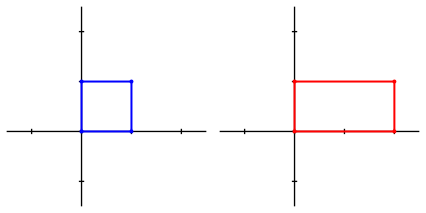
\includegraphics{1_g_polygons}}
\caption{The input square $S$ and the output $T(S)$.}
\label{F:ex:1_g_polygons}
\end{center}
\end{figure}






\end{example}

\csection{Summary}

In this section we determined how to represent any matrix transformation from $\R^n$ to $\R^m$ as a matrix transformation, and what it means for a matrix transformation to be one-to-one and onto.
\begin{itemize}
\item A matrix transformation is a function $T: \R^n \to \R^m$ defined by $T(\vx) = A\vx$ for some $m \times n$ matrix $A$. 
\item A matrix transformation $T$ from $\R^n$ to $\R^m$ satisfies 
\[T(a\vu + b\vv) = aT(\vu) + bT(\vv)\]
for any scalars $a$ and $b$ and any vectors $\vu$ and $\vv$ in $\R^n$. The fact that $T$ preserves linear combinations is why we say that $T$ is a linear transformation. 
\item An $m \times n$ matrix $A$ defines the matrix transformation $T$ via 
\[T(\vx) = A \vx.\]
The domain of this transformation is $\R^n$ because the matrix-vector product $A \vx$ is only defined if $\vx$ is an $n \times 1$ vector. 
\item If $A$ is an $m \times n$ matrix, then the codomain of the matrix transformation $T$ defined by $T(\vx) = A \vx$ is $\R^m$. This is because the matrix-vector product $A \vx$ with $\vx$ an $n \times 1$ vector is an $m \times 1$ vector. The range of $T$ is the subset of the codomain of $T$ consisting of all vectors of the form $T(\vx)$ for vectors $\vx$ in the domain of $T$.
\item A matrix transformation $T$ from $\R^n$ to $\R^m$ is \textbf{one-to-one} if each $\vb$ in $\R^m$ is the image of \emph{at most} one $\vx$ in $\R^n$. If $T$ is a matrix transformation represented as $T(\vx) = A\vx$, then $T$ is one-to-one if each column of $A$ is a pivot column, or if the columns of $A$ are linearly independent.  
\item A matrix transformation $T$ from $\R^n$ to $\R^m$ is \textbf{onto} if each $\vb$ in $\R^m$ is the image of \emph{at least one} $\vx$ in $\R^n$. If $T$ is a matrix transformation represented as $T(\vx) = A\vx$, then $T$ is onto if each row of $A$ contains a pivot position, or if the span of the columns of $A$ is all of $\R^m$.
\end{itemize}




\csection{Exercises}

\be 
\item Given matrix $A=\left[ \begin{array}{ccr} 1& 2 & 1 \\ 1 & 0 & -3 \end{array} \right]$, write the coordinate form of the transformation $T$ defined by $T(\vx)=A\vx$. (Note: Writing a transformation in coordinate form refers to writing the transformation in terms of the entries of the input and output vectors.)

\item Suppose the transformation $T$ is defined by $T(\vx)=A\vx$ where 
\[A=\left[ \begin{array}{ccr} 1&1&-1 \\ 2&1&1 \\ 4&1&4 \end{array} \right].\] Determine if $\vb=\left[ \begin{array}{c} 1\\0\\0 \end{array} \right]$ is in the range of $T$. If so, find all $\vx$'s which map to $\vb$.

\item Suppose $T$ is a matrix transformation and 
\[ T(\vv_1) = \left[ \begin{array}{c} 1 \\ 2 \end{array} \right] \, , \, T(\vv_2) = \left[ \begin{array}{r} -2 \\ 3 \end{array} \right] \]
Find $T(2\vv_1 -5 \vv_2)$.

\item Given a matrix transformation defined as 
\[ T\left( \left[ \begin{array}{c} x_1 \\ x_2 \\ x_3 \end{array} \right] \right) = \left[ \begin{array}{c} 2x_1 -x_3 \\ -x_1 +2x_2 +x_3 \\ 3x_2 - 4x_3 \end{array} \right] \]
determine the matrix $A$ for which $T(\vx) = A\vx$.

\item Suppose a matrix transformation $T$ defined by $T(\vx)=A\vx$ for some unknown $A$ matrix satisfies 
\[ T\left( \left[ \begin{array}{c} 1 \\ 0 \end{array} \right] \right) = \left[ \begin{array}{c} 2\\ 1\end{array} \right] \, \text{ and } \, T\left( \left[ \begin{array}{c} 0 \\ 1 \end{array} \right] \right) = \left[ \begin{array}{r} -1\\ 3\end{array} \right] \, . \] 
Use the matrix transformation properties to determine $T(\vx)$ where $\vx= \left[ \begin{array}{c} x_1\\x_2 \end{array} \right]$. Use the expression for $T(\vx)$ to determine the matrix $A$.

\item For each of the following matrices, determine if the transformation $T$ defined by $T(\vx)=A\vx$ is onto and if $T$ is one-to-one.

\ba
\item $A=\left[ \begin{array}{ccr} 1& 1 & 1 \\ 1 & 2 & -3 \end{array} \right]$

\item $A=\left[ \begin{array}{ccc} 1& 1 & 2 \\ 2 & 2 & 4 \end{array} \right]$

\item $A=\left[ \begin{array}{rcc} 1& 1 & 2 \\ 1 & 2 & 3 \\ -1 & 1 &2 \end{array} \right]$

\item $A=\left[ \begin{array}{cc} 1& 1 \\ 2 & 3 \\ 3 & 0 \end{array} \right]$
\ea

\item Come up with an example of a one-to-one transformation from $\R^3$ to $\R^4$, if possible. If not, explain why not.

\item Come up with an example of an onto transformation from $\R^3$ to $\R^4$, if possible. If not, explain why not.

\item Come up with an example of a one-to-one but not onto transformation from $\R^4$ to $\R^4$, if possible. If not, explain why not.

\item Two students are talking about when a matrix transformation is one-to-one.
\begin{quote}
Student 1: If we have a matrix transformation, then we need to check that $A\vx=\vb$ has a unique solution for every $\vb$ for which $A\vx=\vb$ has a solution, right?
\end{quote} 
\begin{quote}
Student 2: Well, that's the definition. Each $\vb$ in the codomain has to be the image of at most one $\vx$ in the domain. So when $\vb$ is in the range, corresponding to $A\vx=\vb$ having a solution, then there is exactly one solution $\vx$.
\end{quote} 
\begin{quote}
Student 1: But wouldn't it be enough to check that $A\vx=\vzero$ has a unique solution? Doesn't that translate to the other $\vb$ vectors? If there is a unique solution for one $\vb_1$, then there can't be infinitely many solutions for another $\vb_2$.
\end{quote} 
\begin{quote}
Student 2: I don't know. It feels to me as if changing the right hand side could change whether there is a unique solution, or infinitely many solutions, or no solution.
\end{quote}
Which part of the above conversation do you agree with? Which parts need fixing? 

\item Show that if $T$ is a matrix transformation from $\R^n$ to $\R^m$ and $L$ is a line in $\R^n$, then $T(L)$, the image of $L$, is a line or a single vector. (Note that a line in $\R^n$ is the set of all vectors of the form $\vv+c\vw$ where $c$ is a scalar, and $\vv, \vw$ are two fixed vectors in $\R^n$.) 

\item Label each of the following statements as True or False. Provide justification for your response.
\ba
\item \textbf{True/False} The range of a transformation is the same as the codomain of the transformation.

\item \textbf{True/False} The codomain of a transformation $T$ defined by $T(\vx)=A\vx$ is the span of the columns of $A$.

\item \textbf{True/False} A one-to-one transformation is a transformation where each input has a unique output.

\item \textbf{True/False} A one-to-one transformation is a transformation where each output can only come from a unique input.

\item \textbf{True/False} If a matrix transformation from $\R^n$ to $\R^n$ is one-to-one, then it is also onto.

\item \textbf{True/False} A matrix transformation from $\R^2$ to $\R^3$ cannot be onto.

\item \textbf{True/False} A matrix transformation from $\R^3$ to $\R^2$ cannot be onto.

\item \textbf{True/False} A matrix transformation from $\R^3$ to $\R^2$ cannot be one-to-one.

\item \textbf{True/False} If the columns of a matrix $A$ are linearly independent, then the transformation $T$ defined by $T(\vx)=A\vx$ is onto.

\item \textbf{True/False} If the columns of a matrix $A$ are linearly independent, then the transformation $T$ defined by $T(\vx)=A\vx$ is one-to-one.

\item \textbf{True/False} If $A$ is an $m \times n$ matrix with $n$ pivots, then the transformation $\vx \mapsto A\vx$ is onto.

\item \textbf{True/False} If $A$ is an $m \times n$ matrix with $n$ pivots, then the transformation $\vx \mapsto A\vx$ is one-to-one.

\item \textbf{True/False} If $\vu$ is in the range of a matrix transformation $T$, then there is an $\vx$ in the domain of $T$ such that $T(\vx)=\vu$.

\item \textbf{True/False} If $T$ is a one-to-one matrix transformation, then $T(\vx)=\vzero$ has a non-trivial solution.

\item \textbf{True/False} If the transformations $T_1: \R^m \to \R^n$ and $T_2:\R^n \to \R^p$ are onto, then the transformation $T_2 \circ T_1$ defined by $T_2\circ T_1(\vx)=T_2(T_1(\vx))$ is also onto.

\item \textbf{True/False} If the transformations $T_1: \R^m \to \R^n$ and $T_2:\R^n \to \R^p$ are one-to-one, then the transformation $T_2 \circ T_1$ defined by $T_2\circ T_1(\vx)=T_2(T_1(\vx))$ is also one-to-one.

\ea
\ee

\csection{Project: The Geometry of Matrix Transformations}

In this section we will consider certain types of matrix transformations and analyze their geometry. Much more would be needed for real computer graphics, but the essential ideas are contained in our examples. A GeoGebra applet is available at \url{https://www.geogebra.org/m/rh4bzxee} for you to use to visualize the transformations in this project. 

\begin{pactivity} \label{act:1_g_rotation} We begin with transformations that produce the rotated dancing image in Figure \ref{F:Rotate_dance}. Let $R$ be the matrix transformation from $\R^2$ to $\R^2$ defined by 
\[R\left(\left[ \begin{array}{c} x \\ y \end{array} \right] \right) = \left[\begin{array}{lr} \cos(\theta) & -\sin(\theta) \\ \sin(\theta) & \cos(\theta) \end{array} \right]\left[ \begin{array}{c} x \\ y \end{array} \right]. \]
These matrices are the rotation matrices.\index{rotation matrix}
	\ba
	\item Suppose $\theta = \frac{\pi}{2}$. Then 
\[R\left(\left[ \begin{array}{c} x \\ y \end{array} \right] \right) = \left[ \begin{array}{cr} 0&-1 \\ 1&0 \end{array} \right] \left[ \begin{array}{c} x \\ y \end{array} \right]. \]
		\begin{enumerate}[i.]
		\item Find the images of $\vu_1 = \left[ \begin{array}{c} 1 \\ 0 \end{array} \right]$,  $\vu_2 = \left[ \renewcommand{\arraystretch}{1.4} \begin{array}{c} \frac{\sqrt{2}}{2} \\ \frac{\sqrt{2}}{2}  \end{array} \right]$, and $\vu_3 = \left[ \begin{array}{c} 0 \\ 1 \end{array} \right]$ under $R$.

		\item Plot the points determined by the vectors from part i. The matrix transformation $R$ performs a rotation. Based on this small amount of data, what would you say the angle of rotation is for this transformation $R$? 

		\end{enumerate}
	
	\item Now let $R$ be the general matrix transformation defined by the matrix \[\left[\begin{array}{lr} \cos(\theta) & -\sin(\theta) \\ \sin(\theta) & \cos(\theta) \end{array} \right].\] Follow the steps indicated to show that $R$ performs a counterclockwise rotation of an angle $\theta$ around the origin. Let $P$ be the point defined by the vector $\left[ \begin{array}{c} x\\y \end{array} \right] = \left[ \begin{array}{c}\cos(\alpha) \\ \sin(\alpha) \end{array} \right]$ and $Q$ the point defined by the vector $\left[ \begin{array}{c} w\\z \end{array} \right] = \left[ \begin{array}{c} \cos(\alpha+\theta) \\ \sin(\alpha+\theta) \end{array} \right]$ as illustrated in Figure \ref{fig:Rotation_matrix}.
\begin{figure}[h]
\begin{center}
\resizebox{!}{2.0in}{
\includegraphics{Rotation_matrix}}
\caption{A rotation in the plane.}
\label{fig:Rotation_matrix}
\end{center}
\end{figure}
		\begin{enumerate}[i.]
		        \item Use the angle sum trigonometric identities 
		        \begin{align*}
		        \cos(A+B) &= \cos(A) \cos(B) - \sin(A) \sin(B) \\
		         \sin(A+B) &= \cos(A) \sin(B) + \cos(B) \sin(A)
		        \end{align*}
		        to show that
    \begin{align*}
    w &= \cos(\theta)x - \sin(\theta)y \\
    z &=  \sin(\theta)x + \cos(\theta)y.
    \end{align*}

	\item Now explain why the counterclockwise rotation around the origin by an angle $\theta$ can be represented by left multiplication by the matrix 
            \[\left[ \begin{array}{rr} \cos(\theta) & -\sin(\theta) \\ \sin(\theta) & \cos(\theta) \end{array} \right].\]
        
	\end{enumerate}
		
	\ea
	
\end{pactivity}

Project Activity \ref{act:1_g_rotation} presented the rotation matrices. Other matrices have different effects. 

\begin{pactivity} \label{act:1_g_shear} Different matrix transformations 
\ba
\item Let $S$ be the matrix transformation from $\R^2$ to $\R^2$ defined by 
\[S\left(\left[ \begin{array}{c} x \\ y \end{array} \right] \right) = \left[ \begin{array}{cr} 1&0.5 \\ 0&1 \end{array} \right]\left[ \begin{array}{c} x \\ y \end{array} \right].\]

Determine the entries of the output vector $S\left(\left[ \begin{array}{c} x \\ y \end{array} \right] \right)$ and explain the action of the transformation $S$ on the dancing figure as illustrated in Figure \ref{F:Shear_x_Dance}. (The transformation $S$ is called a \emph{shear}\index{shear} in the $x$ direction.)
\begin{figure}[ht]
\begin{center}
\resizebox{!}{1.5in}{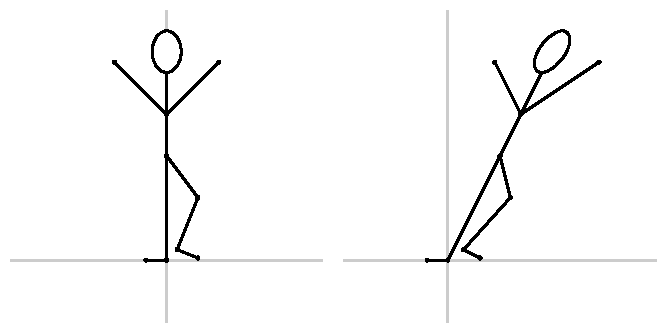
\includegraphics{1_g_shear_x}} 
%\resizebox{!}{1.5in}{\includegraphics{Dancing_man_original}} \hspace{0.5in}  \resizebox{!}{1.5in}{\includegraphics{Dancing_man_shear_x}}
\caption{A dancing figure and a sheared dancing figure.}
\label{F:Shear_x_Dance}
\end{center}
\end{figure}
%\resizebox{!}{1.0in}{\includegraphics{1g_dancing_man_shearx}}


\item Let $C$ be the matrix transformation from $\R^2$ to $\R^2$ defined by 
\[C\left(\left[ \begin{array}{c} x \\ y \end{array} \right] \right) = \left[ \begin{array}{cr} 0.65&0 \\ 0&0.65 \end{array} \right]\left[ \begin{array}{c} x \\ y \end{array} \right].\]

Determine the entries of the output vector $C\left(\left[ \begin{array}{c} x \\ y \end{array} \right] \right)$ and explain the action of the transformation $C$ on the dancing figure as illustrated in Figure \ref{F:Contract_Dance}. (The transformation $C$ is called a \emph{contraction}\index{contraction}.) How would your response change if each $0.65$ was changed to $2$ in the matrix $C$? 
\begin{figure}[ht]
\begin{center}
\resizebox{!}{1.0in}{\includegraphics{1_g_dancer_contract}}
%\resizebox{!}{1.5in}{\includegraphics{Dancing_man_original}} \hspace{0.5in}  \resizebox{!}{1.5in}{\includegraphics{Dancing_man_scale}}
\caption{A dancing figure and a contracted dancing figure.}
\label{F:Contract_Dance}
\end{center}
\end{figure} 

\ea

\end{pactivity}

So far we have seen specific matrix transformations perform a rotations, shears, and contractions. We can combine these, and other, matrix transformations by composition to change figures in different ways, and to created animations of geometric figures. (As we will see later, combining transformations needs to be done carefully in order to obtain the result we want. For example, if we want to first rotate then translate, in what order should the matrices be applied?)


